\chapter{Project Resource Management}

This section of the report details the testing process and resource allocation for the project.

\section{WBS for Testing Process}

To allocate resources properly, we begin by creating a Work Breakdown Structure (WBS) for testing, as shown in Table \ref{tab:wbs_testing}.

\begin{table}[h]
\centering
\begin{tabular}{|>{\raggedright\arraybackslash}p{1cm}|>{\raggedright\arraybackslash}p{5cm}|>{\raggedright\arraybackslash}p{2cm}|>{\raggedright\arraybackslash}p{5cm}|}
\hline
\rowcolor{lightgray} \textbf{Index} & \textbf{Task} & \textbf{Time} & \textbf{Deliverable} \\
\hline
1 & Write Test Plan & 1 week & Test Plan Document \\
\hline
1.2 & Unit Testing & 1 week & Unit Test Reports \\
\hline
1.3 & Integration Testing & 2 weeks & \\
\hline
1.3.1 & Registration Module & 5 days & Integration Test Reports for Registration \\
\hline
1.3.2 & Tracking Module & 5 days & Integration Test Reports for Tracking \\
\hline
1.3.3 & Incentives Module & 4 days & Integration Test Reports for Incentives \\
\hline
1.4 & System Testing & 1 week & System Test Reports \\
\hline
1.5 & User Acceptance Testing & 1 week & User Acceptance Test Reports \\
\hline
\end{tabular}
\caption{Work breakdown structure for testing}
\label{tab:wbs_testing}
\end{table}

\section{Responsibility Assignment Matrices (RAM)}

\begin{figure}[ht]
    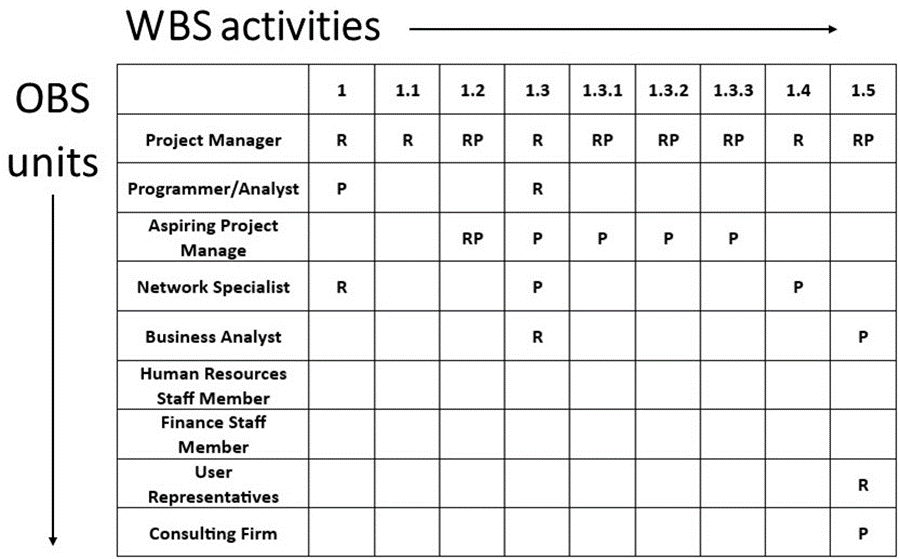
\includegraphics[width=\textwidth]{images/ram.png}
    \caption{RAM Matrix}
    \label{fig:ram}
\end{figure}

\subsection*{RACI Chart for Testing Tasks}

To clarify roles and responsibilities for testing tasks, the following RACI chart has been created:

\begin{longtable}{|p{3cm}|p{2cm}|p{2cm}|p{2cm}|p{2cm}|p{1cm}|p{1cm}|}
\caption{RACI Chart for Testing Tasks}
\label{tab:raci_testing} \\
\hline
\rowcolor{lightgray} \textbf{Task} & \textbf{Project Manager} & \textbf{Programmer} & \textbf{Network Specialist} & \textbf{Business Analyst} & \textbf{Users} & \textbf{Firm} \\
\hline
\endfirsthead
\caption[]{(continued)} \\
\hline
\rowcolor{lightgray} \textbf{Task} & \textbf{Project Manager} & \textbf{Programmer} & \textbf{Network Specialist} & \textbf{Business Analyst} & \textbf{Users} & \textbf{Firm} \\
\hline
\endhead
\hline
\endfoot
\hline
\endlastfoot
Write Test Plan & R & R/C & C & C & I & R/C \\
\hline
Unit Testing & R & R/C & C & C & I & R/C \\
\hline
Integration Testing & R & R/C & R/A & R/C & I & R/C \\
\hline
Registration Module & R & R/C & R/A & R/C & I & R/C \\
\hline
Tracking Module & R & R/C & R/A & R/C & I & R/C \\
\hline
Incentives Module & R & R/C & R/A & R/C & I & R/C \\
\hline
System Testing & R & R/C & R/A & R/C & A & R/C \\
\hline
User Acceptance Testing & A & R/C & C & C & A & R/C \\
\hline
\end{longtable}

\section{Weekly Data}

The following table presents the resource allocation for each week during the testing phase.

\begin{table}[h]
    \centering
    \caption{Weekly Data}
    \label{tab:weekly_data}
    \begin{tabular}{|l|c|c|c|c|}
    \hline
    \rowcolor{lightgray} \textbf{Week} & \textbf{Senior Testers} & \textbf{Junior Testers} & \textbf{User Group} & \textbf{Managers} \\
    \hline
    First week  & 1 & 0 & 2 & 0 \\
    \hline
    Second week & 1 & 0 & 0 & 0 \\
    \hline
    Third week  & 1 & 2 & 0 & 0 \\
    \hline
    Fourth week & 1 & 2 & 4 & 0 \\
    \hline
    Fifth week  & 1 & 2 & 4 & 3 \\
    \hline
    Sixth week  & 1 & 2 & 4 & 3 \\
    \hline
    \end{tabular}
\end{table}

\section{Resource Histogram}

To visualize the resource allocation over time, a resource histogram is provided in Figure \ref{fig:rhst}.

\begin{figure}[ht]
    \centering
    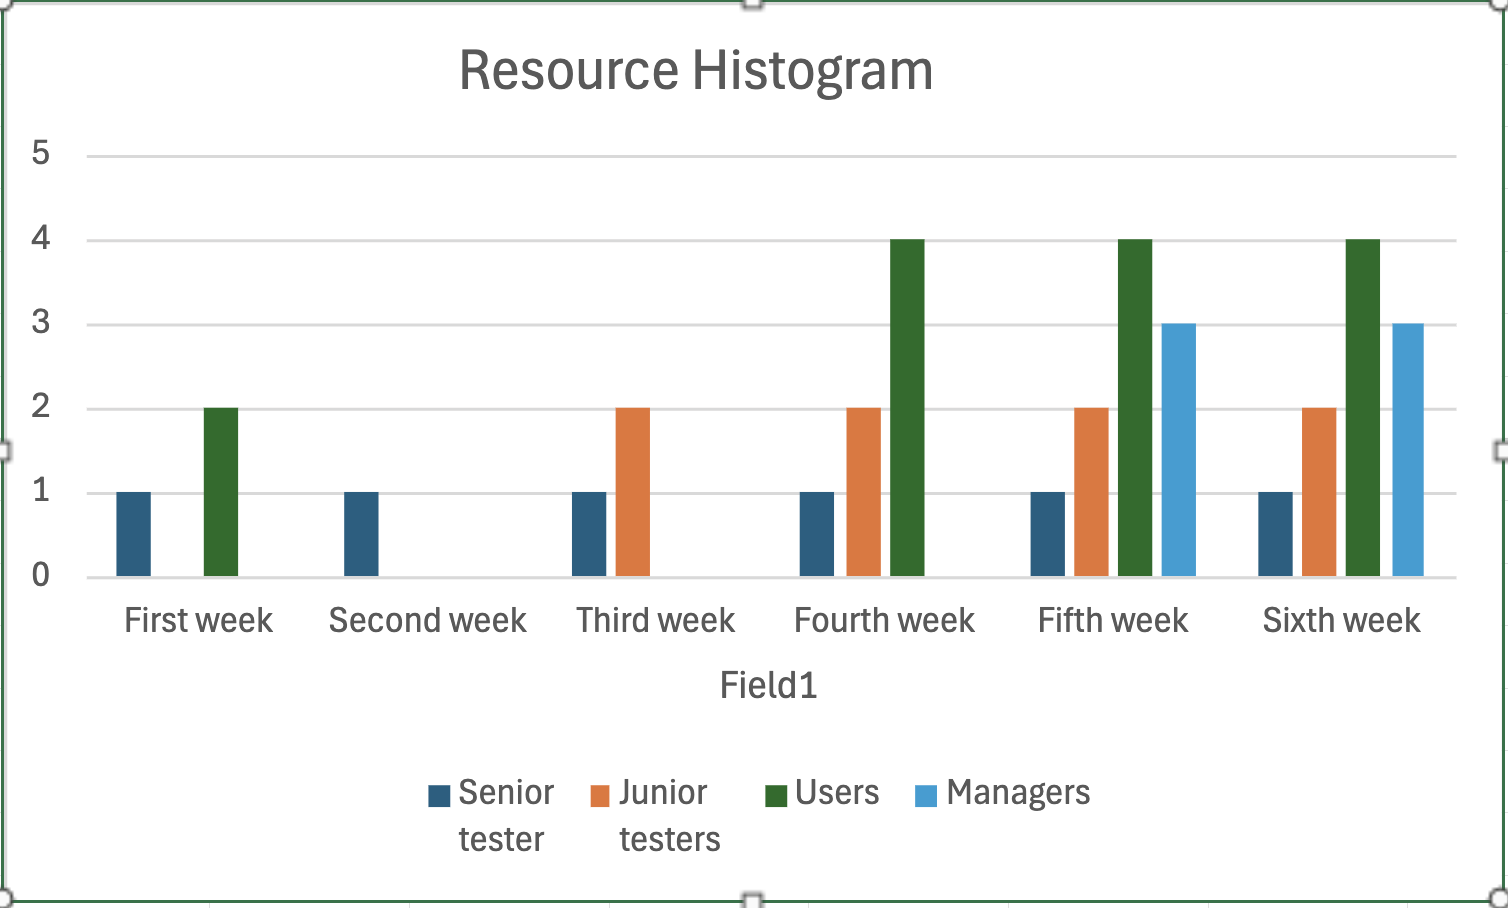
\includegraphics[width=\textwidth]{images/Resource Histogram.png}
    \caption{Resource Histogram}
    \label{fig:rhst}
\end{figure}

\FloatBarrier
\newpage